% !Mode:: "TeX:UTF-8"

\chapter{绪论}

\section{研究课题的来源、背景和意义}

本研究课题来源于哈尔滨工业大学和中国移动联合实验室承接的基于黑龙江省移动用户数据开展多方面的研究和分析。本研究需要解决的问题是通过移动提供的数据,对哈尔滨市用户的职业、家庭特征进行分析,绘制出用户画像,为后续精准营销、城市规划等研究打下数据基础。

\section{国内外与课题相关研究领域的研究进展及成果}

\subsection{大数据及其相关理论和应用的发展概况}
\label{sec:bd_dev}

全球互联网时代的到来,不管是早期的个人电脑、移动电话,甚至是目前发展势头正盛的各种接入互联网的设备形成的物联网,虽然带给人们越来越多的便携性,但各方面人士对偌大的全球性网络中产生的数据提出相当多的问题。除了个人隐私、数据归属等使用权以及相关法律层面的问题,开发人员不能逃避的一个重要问题则是超大规模数据的存储、处理和查询。

根据国际数据公司(IDC,International Data Corporation)的预测\cite{data_count},由于 5G 的商用化在中国国内逐渐铺开,企业和用户的设备产生的数据将会成为中国数据的主流,数据量和数据市场将产生跨越式增长,在 2023 年左右达到 40ZB ($1ZB \approx 10^{12}GB$)。

飞速增长的数据量,无论单台计算机的存储能力、计算速度达到何种水平,在数以 PB 计的数据量面前,都不足以应对。同时,单机的价格相对于其性能并不是线性增加的,昂贵的单机服务器使团体或者公司无法负担处理如此庞大数据量的成本,二十世纪初的大数据也只能被丢弃。

首先解决该问题的是谷歌,2003 年谷歌发表了三篇技术论文\cite{gfs},分别是解决了存储大规模数据的 GFS(Google File System,谷歌文件系统),解决了大规模计算的 MapReduce 方法,以及解决了实时查询的 BigTable 系统。之后雅虎公司推出了 Hadoop 平台及其生态,被 Apache Software Foundation 公司引入开源应用。 其中,最有价值的 GFS 相关的论文使得 HDFS(Hadoop Distributed File System,Hadoop 分布式文件系统)的开源实现成为了目前绝大部分大数据平台的基石。

\begin{figure}[htpb]
    \centering
    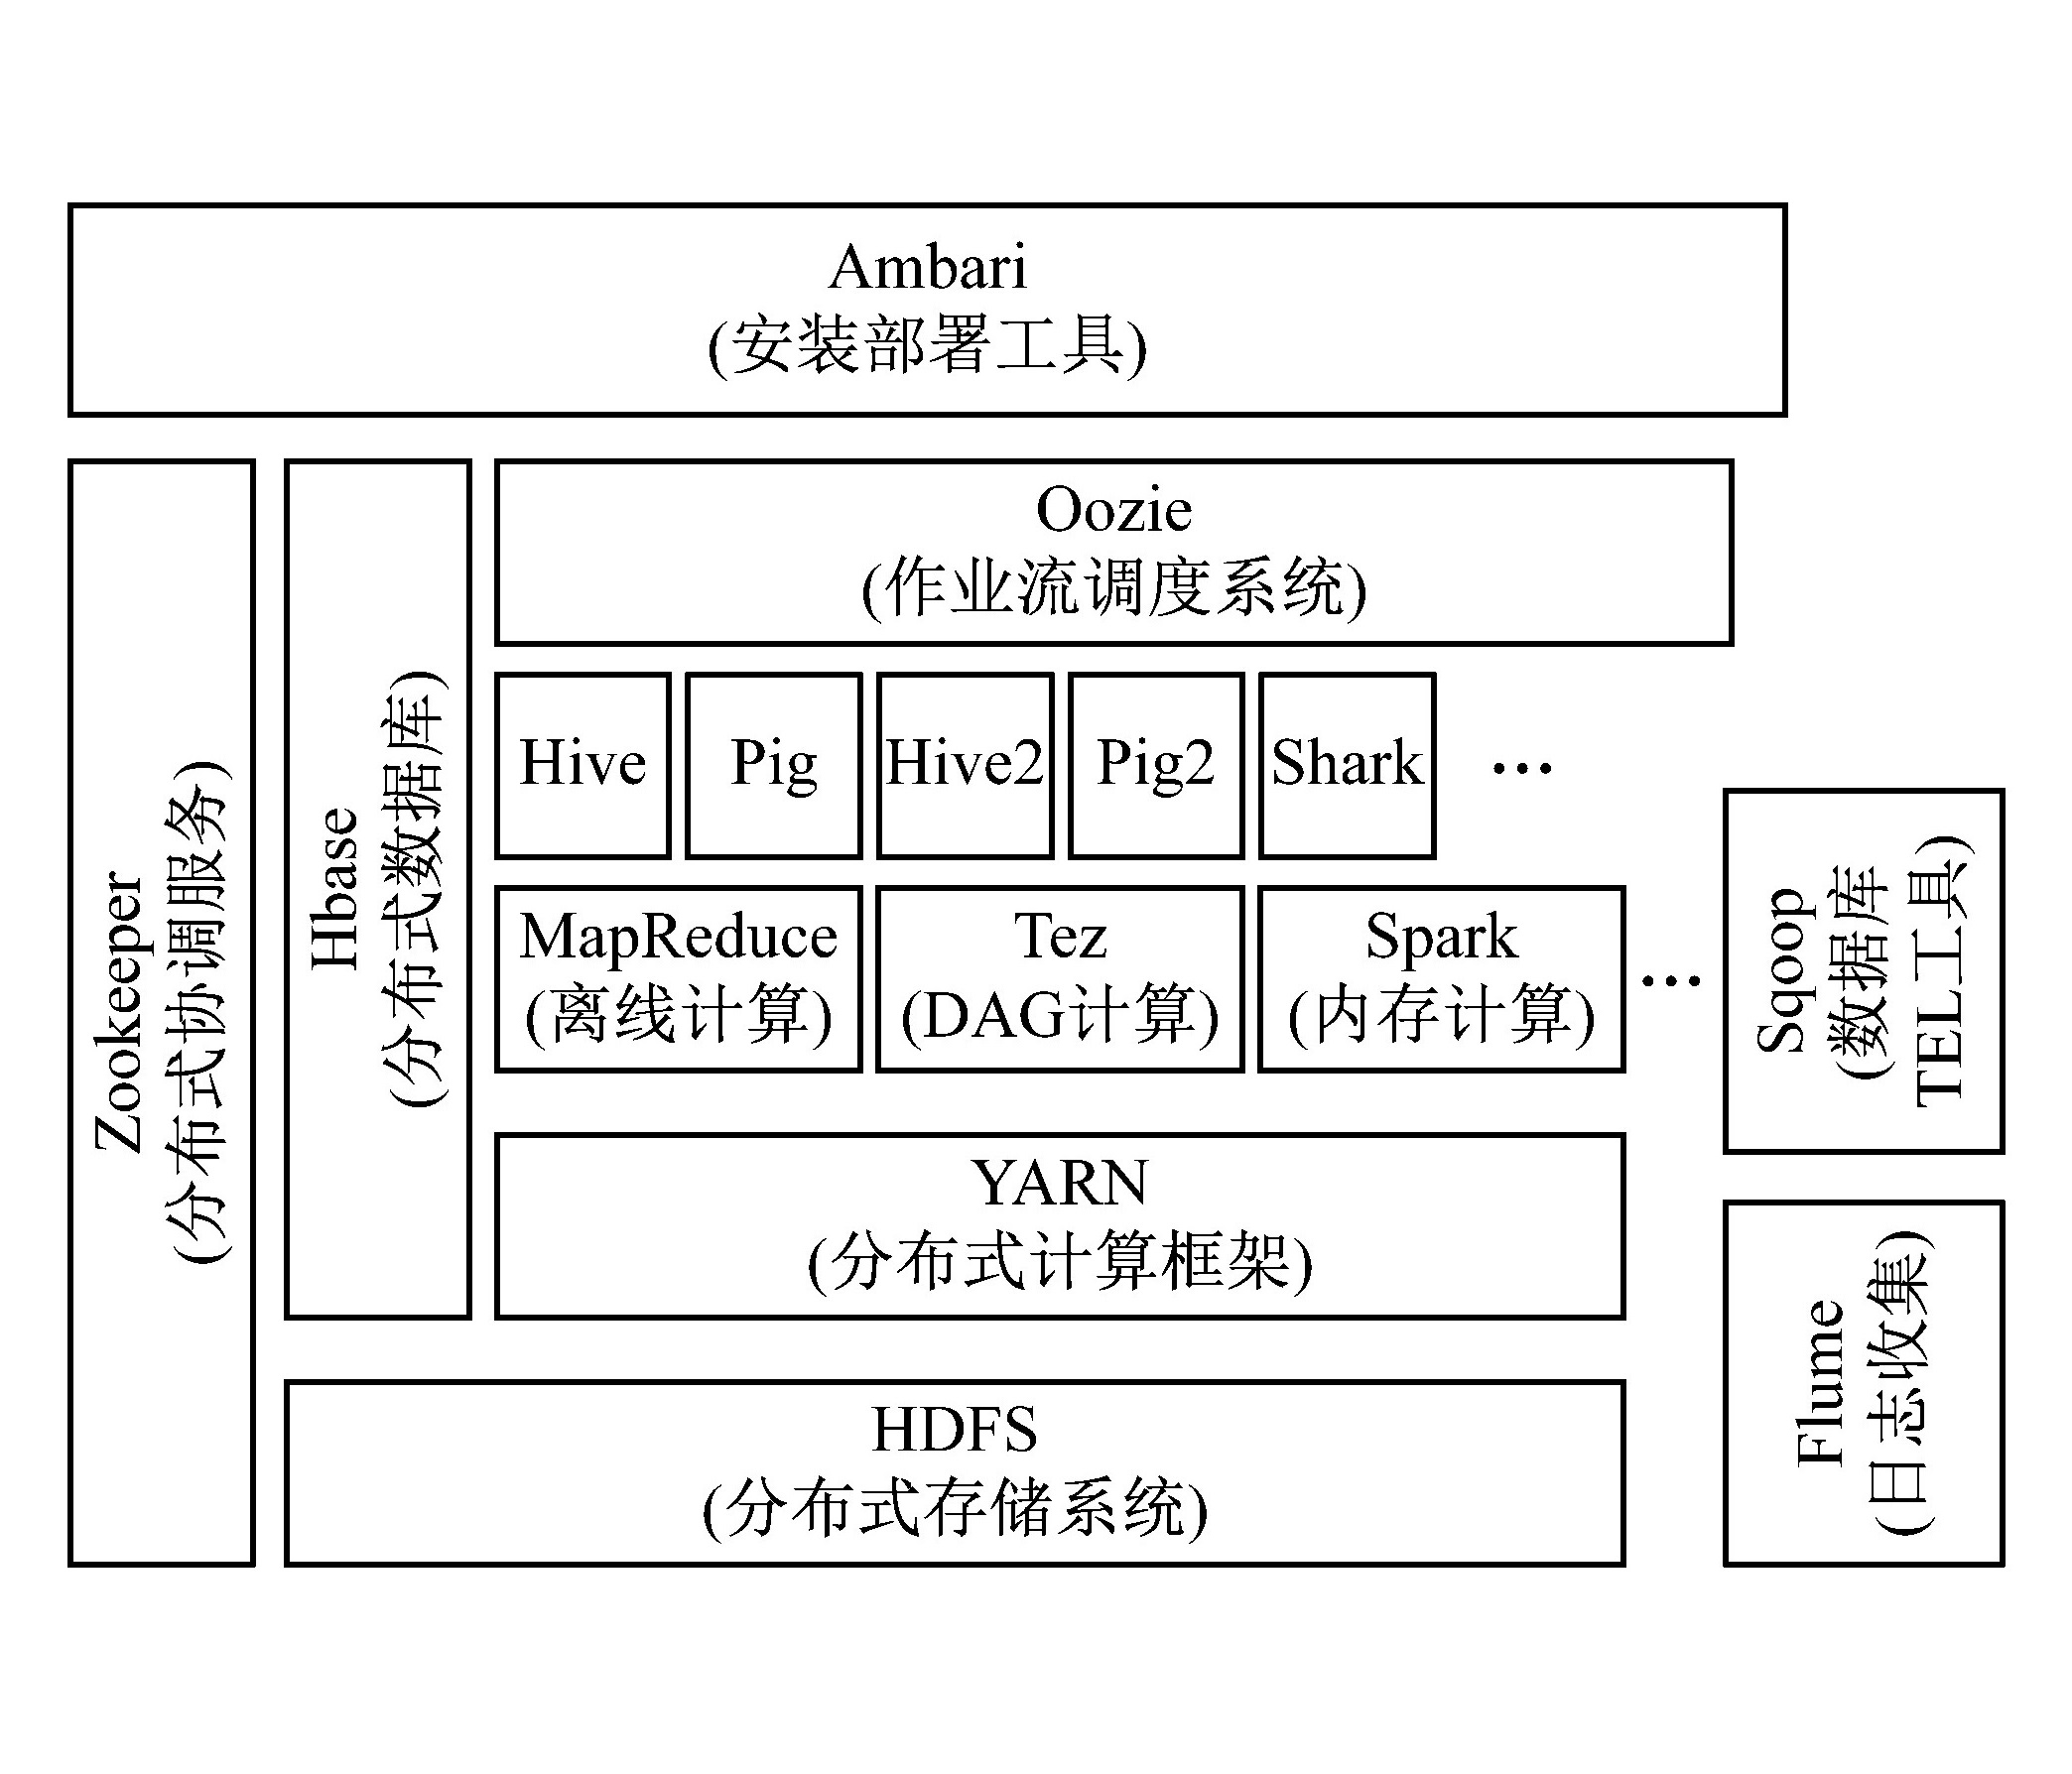
\includegraphics[width = 0.8\textwidth]{hadoop.jpg}
    \caption{Hadoop 生态系统}
    \label{fig:hadoop}
\end{figure}

如图 \ref{fig:hadoop} 所示,最底层的 HDFS 分布式文件存储系统是整个大数据领域的基础,通过切分超大文件,实现了一个多机保存、备份以及高容错的大数据文件系统。HDFS 只上的是 Yarn(全称 Yet Another Resource Manager),主要由于 Hadoop 1.0 版本中的重大架构缺陷,导致任务调度系统(JobTracker)承担了太多诸如资源调度、异常监控、接受任务等不同且复杂的任务,于是行业将 JobTrakcer 的任务拆分开来,形成了建立在 HDFS 上的新的调度系统,能够兼容更多的计算框架,如本研究使用的 Spark 以及同样用 DAG 优化的 Tez 等。

MapReduce 则是一种计算模型,通过一次 Map 操作生成 key-value 键值对,以及第二次 Reduce 操作对所有键值对进行规约,得到最终的结果。而 MapReduce 如此暴力的实现方法被数据库领域的专家 David J. DeWitt\cite{mr_back} 在一篇著名论文 \emph{MapReduce: A Major Step Backwards} 中指责谷歌在大数据的计算上即 MapReduce 方法放弃了数据库领域中的优秀理论和方案,选择了简单粗暴的解决办法。不久,加州大学伯克利学院的 AMP 实验室则推出取 MapReduce 和数据库中精华的 Spark 平台,通过 DAG(有向无环图)解决了多次机器学习、聚类算法中多次迭代的麻烦问题,以及稳定的 Spark Streaming,MLlib 等拳头产品,使 Spark 平台及其套件,成为众多公司的选择。

\begin{figure}[htpb]
    \centering
    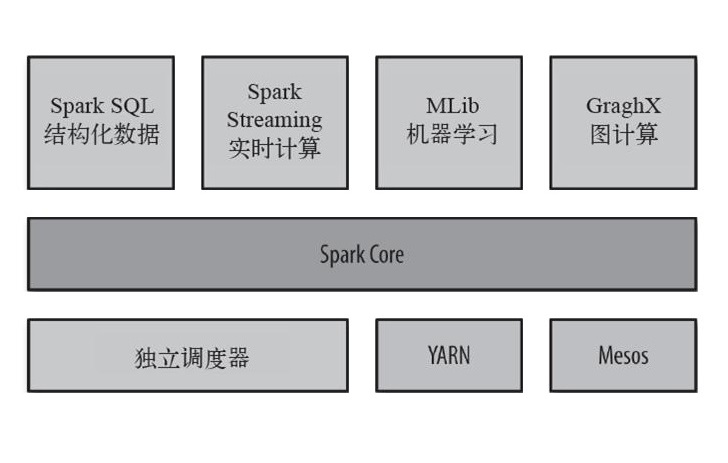
\includegraphics[width = 0.8\textwidth]{spark.jpg}
    \caption[fig:spark]{Spark 生态系统}
    \label{fig:spark}
\end{figure}

如图 \ref{fig:spark} 所示,整个 Spark 生态系统中的核心是 Spark Core,从基于 HDFS 的 YARN 框架、HBase、Hive 数据库等中读取数据,通过独立调度器(Standalone)、YARN 和 Mesos 调度任务(Job),然后完成 Spark 程序,或者通过 spkar-shell/spark-submit 等命令行工具,批量运行或提交任务,再利用基于 Spark Core 的 Spark Stream 完成实时计算、MLLib 实现机器学习以及 GraghX 进行图形计算提高程序运行速度。

除此之外,与只推荐用 Java 编写 MapReduce 程序不同,Spark 能够和多种动态或静态语言配合,如 Python、Scala、Java,甚至能够启用 spark-shell 命令行工具,使用 Scala 语言进行交互式查询,灵活便捷。Spark 还支持更复杂的操作,除开类似 MapReduce 的固定的生成 key-value 键值对的方法,Spark 基于 RDD 模型(Resilient Distributed Datasets,抽象弹性分布式数据集),只需要承担非常小的代价,就能实现如 SQL 中的 join、union 等高阶方法,以及流式查询功能。

\subsection{手机信令数据与职住特分析的相关理论和发展概况}

2020 年 9 月,中国互联网络信息中心(CNNIC)第 46 次发布了《中国互联网络发展状况统计报告》\cite{2020_mobile},截止 6 月底,中国已经形成了 9.4 亿规模的网民群体,移动互联网用户规模更是达到了 13.19 亿人,同时“中华人民共和国国民经济和社会发展第十三个五年规划纲要”中首次明确指出 2020 年的互联网普及率计划,要将移动宽带的普及率提升到 85\%,如此庞大的用户数量,必然会产生超大规模的用户数据,客户在日常的手机使用中,会产生诸如基站连接记录、手机应用流量使用记录、点对点通话记录、短信记录等。

其中,用户手机接受信号产生的基站连接记录的数据成为一个重点分析对象,连接数据能够模糊推断出用户的位置,根据这一点,2017 年孔扬鑫\cite{kong_people}采用了轨迹行为特征的判定算法,基于 MapReduce 分布式计算模型,基于用户的基站连接数据,分析基站连接的消失点、消失时长、用户停留点、用户工作地点与家庭住址的平均距离,计算出用户进出城的人口流动的统计数据,再基于基站与县区之间的关系,判断用户的通勤起终点所属区域,最终得到用来反映城镇间、工作地居住地间的人口流动的状态转移序列。

由于城区的范围都比较大,因为基站的覆盖面积广而导致位置的推算的误差并不能显著的影响用户所处城镇的结果。但如果需要精确到城区内部的定位,或者对用户未来位置的推断,就必须要把基站范围导致的误差考虑在内。北京邮电大学 2019 年刘奕杉\cite{liu_pos_forecast}则是基于用户连接基站的记录产生的状态转移序列,构建了位点转移的语义序列,再利用 TS-RNN(Three-layer Symmetircal Recurrent Neural Network,三层对称卷积神经网络)提取出转移特征值,实现了更精准的用户活动区域获取以及位置预测。

常在春\cite{chang_job_space}在延庆区职住空间关系分析一文中同样利用 Spark 大数据平台,首先对延庆地区的手机信令数据做一个初步筛选,主要针非过境、常驻、非固定设备用户的工作以及居住地位置的分析,然后使用核密度法得到多个工作地和居住地对应的基站的信息,最终实现用户对工作地点及居住地点的信息推算,并且对延庆区的通勤、工作地使用情况、居住地使用情况等进行描述和分析。

\subsection{城市功能区与用户行为目的和职住特征分析研究进展及成果}
\label{sec:city_dist}

需要分析用户的职业居住的特征分析,就必然不能绕开对用户所处位置的功能语义分析,即用户处于什么目的而移动到该区域。为了能够大致描述用户目的,就需要对城市进行功能区划分。由文献\cite{yang_beijing_district}可知,杨振山等人融合北京市移动电话信令数据以及网络地图 API 提供的 POI(Point of Interest,兴趣点),通过计算单位数量 POI 的人口密度、标准化的单位面积 POI 密度以及类内散度矩阵等特征,对栅格化后的北京市推断所有区块的主导功能类型,得到如北京市功能区比率分布,居住和餐饮、娱乐、服务等工作区块分布特点,以及区块的日夜活跃等特点。

除了对城市进行栅格化城区对每个区块进行分析,还有根据城市主要路网对市区进行一个大致上的划分,福建农林大学毋亭在对泉州市\cite{quanzhou}按照路网信息划分出不规则的网格作为研究单元,同时提出按照多个属性如群众对区域类型的认知度(如对大学的认知度较高、对一般商店认知度较低)、该类型覆盖的面积对区块进行权重赋值,基于该种划分和权重法,再加上核密度估计法,完成对不同功能区的识别和划分,最后通过对泉州市地图进行对比,验证准确率。

本文研究用户的职住画像,需要根据城市中职住区域的分布进行参数上的调整,文献\cite{wang_beijing}对北京市的职住空间分布进行定量的研究,通过分析北京市三十余天一亿多条的基站的链接数据,根据北京市的路网结构情况,综合运用职住偏离度、空间错误指数和职住分离率等特征,研究城市功能区分布规律和匹配特点,为本研究对哈尔滨市的研究提供了参考。

\subsection{大数据下的职住空间聚类算法的分析和改进}

本研究需要对城市的功能区进行聚类,得到用户移动语义,针对哈尔滨市 67 万余条城市兴趣点信息,需要一个高效、准确的聚类算法。如章节 \ref{sec:bd_dev} 所言,基于 Spark Core 这个核心,以及拆分成不同组件的调度器、Mesos 等结构,Spark 能够灵活的提供非常多种无监督聚类以及有监督的机器学习等操作。比如 Spark MLLib 库中提供的 K-Means 算法,通过基于 HDFS 的 Yarn 框架,读取分布式数据,采用类似 Map 的方法生成若干对键值对,Spark Core 再将这些键值对分配到各个节点上,分布式地完成 K-Means 算法,该算法充分利用了 Spark 的高弹性分布式数据集,在高扩展、速度快的条件下,完成多种无监督聚类算法。

文献\cite{zhang_poi},东北大学张景奇等人指出,中国 2010 年到 2019 年截止,知网上有 625 篇关于 POI 兴趣点数据研究的文章,特别是在 2017 年之后发生了爆炸式的增长,而关于 POI 兴趣点的分析方法主要是空间自相关分析、核密度估计以及 DBSCAN 聚类算法。作者的研究表明,兴趣点大数据对城市功能区布局、空间结构以及发展规律的分析都起到一个非常重要的影响。

比如文献\cite{shao_jiejing}就通过背景和上海的兴趣点大数据以及不同的聚类算法,分析北京市和上海市的街道元素,从而得到两市的城市舒适度评价。文献通过路网数据将城市进行语义上的分隔,通过街景元素的可视数量的占比加上 K-Means 聚类分析,将街景分成 29 类并进行相关性分析以及舒适度评价。利用路网数据进行语义分割加上 K-Means 街景分类为本研究的街区分类提供了聚类路线上的参考。

不过本研究的街区划分颗粒度较细,POI 兴趣点的数量较多,使用一般的 Kmeans 聚类算法在时间复杂度上不够优秀,需要寻找优化方法。比如文献\cite{li_minibatch}中,为了提高室内 WLAN 定位的算法性能和准确度,希望通过先聚类再采用 XGBoost 分类算法确定准确位置,为了解决超大规模数据量的问题,文献采用大数据优化的 Minibatch K-Means 聚类算法,降低了数据维数、提高了运算速度的同时,仍然保持了较高的准确率,不失为一个大数据下的聚类优化算法。

\subsection{基于手机信令的用户特征画像分析相关研究进展及成果}

文献\cite{wang_huaxiang}没有着眼于兴趣点驻留偏好,而是通过手机信令数据,刻画出用户的高聚集点,刻画出两点一线、双核心、均匀分布等轨迹类型,再根据用户的其他特征,描述和推测用户的职业类型(如学生、退休老人、技术工种等)、爱好属性,以及年龄层分布等相关信息。文献中值得借鉴的方面,包括数据的预处理,作者首先对原始数据进行均匀间隔采集处理、清楚无效和重复数据、分隔时间段,然后基于 DBSCAN 聚类算法改进出一种高簇聚类法得到用户的如居住点、工作地、娱乐场所等核心点。

除了基站连接数据的应用,文献\cite{zheng_game}中利用游戏类 APP 流量数据与其他 APP 流量数据的比率,同时处理用户的短信费用、流量套餐极其费用以及手机连接流量时发送的请求推算出手机的大致平台,通过上述处理后的数据,划分出不同年龄层、不同消费等级、不同的消费行为以及不同的消费心理等,细分用户群,准确把握客户价值从而实现精确营销。其中对不同 APP 相关数据运用对本研究处理用户 APP 流量数据的处理有一定的引导和启发效果。

\subsection{存在的不足或有待深入研究的问题}
\label{sec:buzu}

章节 \ref{sec:city_dist} 中提到了基于路网的城市区块划分,如文献 \cite{xue_liaoning_dist} 中以辽宁省本溪市为例,配合核密度法、公众认知度以及区块大小等因素推算出城市功能区分类,如图 \ref{fig:liaoning}。但是路网的颗粒度太粗的同时,一些区块如小学校、商场等建筑,并没有用街道去划分界限,导致并不能够较为准确地判断该区域的功能区类型。 

\begin{figure}[htpb]
    \centering
    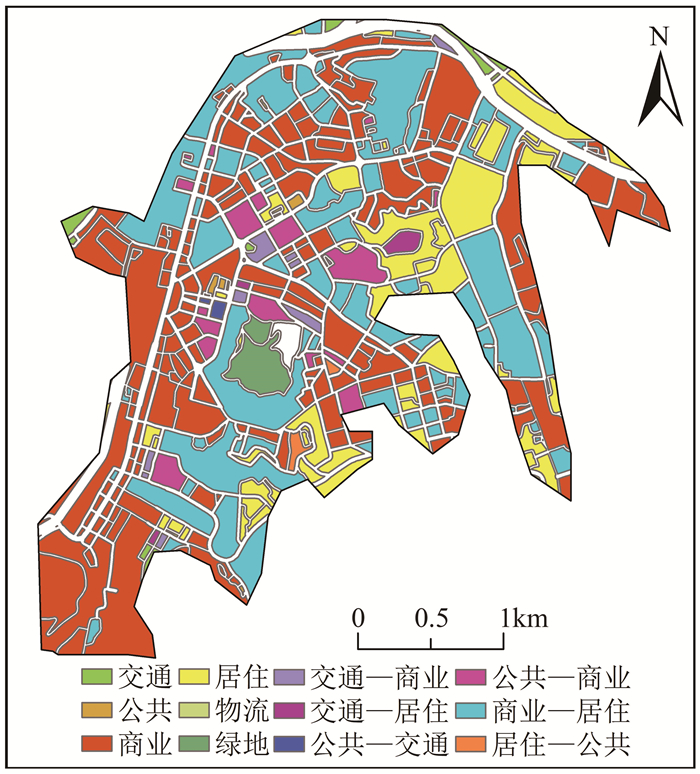
\includegraphics[width = 0.5\textwidth]{liaoling_dist.jpg}
    \caption{辽宁省本溪市功能区分布图}
    \label{fig:liaoning}
\end{figure}

如果采用文献\cite{yang_beijing_district}的中提到的的通过栅格化城市来描述区块的类别,虽然可以在较细颗粒度的情况下分析功能区,但是同样需要注意的是,该方法需要考验研究人员对栅格长宽的确定,不同大小的栅格以及栅格兴趣点 POI 的数据量都会称为影响区块分类的因素。

上面提到的文献中,描述的用户画像多为工作地、居住地、通勤时间等交通、城区规划方向的标签,而缺少对用户是否有工作、工作时长、是否经常加班、使用 APP 偏好等画像的分析,这些都是有待本研究深入研究的问题。

\section{本课题的主要研究内容概述}

\subsection{数据分析与可用性判断}

本研究首先要对中国移动提供的数据进行统一的描述与判断,比如用户与基站的连接数据,每天有多少条用户,用户唯一标识符使用手机号码还是 ICCID(Integrate Circuit Card Identity,集成电路卡识别码即手机 SIM 卡卡号),连接时间的数据类型,字符串或是到 1970 年 1 月 1 日零点的毫秒数等,都需要研究人员仔细分析、做下标记,为之后的研究和处理提供数据轮廓。

同时提取重要的信息表,比如研究用户 APP 偏好画像时,用户 APP 使用数据表和 APP 的描述信息表(如类别,名称,唯一标识符等)都是关键数据,需要认真筛选并且做出数据流向图为数据的分析开发奠定基础。

\subsection{大数据下 K-Means 聚类方法的分析和优化}

由于 K-Means 的时间复杂度为 $O(KNTD)$,K 表示聚类数量,N 表示被聚类元素数量,T 表示迭代次数,D 表示距离的计算复杂度,具体为样本的特征数量,总体来说是关于被聚类元素的总数量的时间复杂度。为了平衡执行速度和聚类效果,本研究会比较两种 K-Means 优化算法,K-Means++ 和 Minibatch K-Means,从中选出一个各方面均衡的聚类优化方法。

\subsection{哈尔滨市栅格化处理以及对栅格化后的街区类型分析}
\label{sec:xu:block_type}

综合章节 \ref{sec:buzu} 中提到诸多因素,本研究选择颗粒度更小的栅格化城市处理方式。首先通过爬虫程序获取哈尔滨市区的兴趣点信息表,然后按照不同的标准对城市进行栅格化处理。对于每次栅格化后的城市,根据每一格中 POI 兴趣点的数量和类型,建立不同的模型来表示这一格中的兴趣点分布情况,接着做一次 K-Means 聚类分析,得到哈尔滨市城市功能区类型的聚类结果。

对于每一次聚类结果,对比哈尔滨市真实的城市地图,分析和判断聚类结果的准确性,调整栅格的长宽,以及描述 POI 兴趣点在每一个栅格中的模型,以求达到一个类型精准、大小合适的城市功能区类型分布描述。

\subsection{大数据系统及其套件的分析和比较}

目前较为常用的大数据计算框架有:基于最早由雅虎开源的 MapReduce 流程;基于 HDFS 和 MapReduce 但内部进行优化同时提供了方便编写成 SQL 语句的 Hive 数据库;以及通过 DAG 和内存优化的 Spark 计算框架。本研究中的数据部分保存在 HDFS 和 Hive 中,为了提高计算速度、降低程序复杂度,该研究会对比这三种工作流程,并做出适合本项目的选择配比。

\subsection{基于手机信令数据的用户驻留点判定}
\label{sec:stop_point}

原始数据中并不包含用户位置的准确信息,只能通过用户对基站的连接序列来确定用户的驻留点偏好。而基站的覆盖范围很广,如一整天待在哈尔滨工业大学一校区十八公寓的学生,能连接到西北方向曲线街附近的一个基站,间隔约 500 米,所以为了更为准确的描述用户的位置信息,需要对基站连接序列进行去震荡处理。对于一个序列 $A \to B \to C$,通过一定的判断标准,认定 B 点属于漂移点而不是用户真正所前往的点,从而将其剔除,提高用户驻留点结果的可信度。

\subsection{基于手机信令数据的不同时间段用户访问街区类型偏好}

排除掉非个人用户,哈尔滨市一天月 400 万用户产生 4000 余万条约 1.2TB 左右的基站连接数据量,而该研究需要讨论一定时间段,如一个月内的基站连接情况,如此大规模的数据需要研究人员编写大数据计算程序如 MapReduce 或 Spark 任务进行分析。利用章节 \ref{sec:stop_point} 提到的驻留点判定方法,筛选出可信的用户位置信息,合并给定时间段内的数据。

同时为了准确表达用户画像,还要将基站连接频次按四个时间段:工作、午休、加班、晚休进行统计,最后得到四个时间段中访问的不同的基站序列,再根据章节 \ref{sec:xu:block_type} 提出的栅格化城市功能区,统计出用户在四个时间段对不同类型区块的访问偏好度,最终得到用户的移动语义。

\subsection{基于手机应用数据的不同时间段用户手机应用类型偏好}

类似于用户基站连接数据,用户的手机应用使用数据条数即使按天计算也是非常的庞大,同样需要编写基于大数据框架下的程序来统计用户在不同时间段对实际应用类型的偏好。首先需要认清楚应用唯一标识符意义,然后根据在应用商城中爬取的数据,一一对应获得不同应用的详细信息,如一级类型、二级类型、评分、用户下载量等。接下来根据用户在不同时段使用某个应用的流量数据,统计用户每天在四个时间段对某类应用的偏好,最终得出用户在一段时间内对某类应用的偏好,由街区访问偏好和应用使用偏好进而刻画用户画像。

\subsection{基于手机通信数据的用户社交习惯和偏好分析}

同样的,还有中国移动公司提供的用户通信数据,包括电话呼叫和短信收发。分析数据结构做出大众的描述性统计,根据结果推算用户在社交中的地位,如接拨电话、收发短信的比率,通话对端归属地比率,通信的总时长,超过某个时长的天数等等,最终得到关于用户社交的习惯和评价。

\subsection{基于手机信令数据的用户职业特征与家庭特征分析}

经过上述一系列处理,最终可以得到用户在四种时间段:工作、午休、加班、晚休对于驻留点的偏好、手机应用使用的偏好,连续一段时间内社交地位(拨入和拨出比率)等,从而刻画用户关于职业的特征。包括用户是否有一个稳定通勤路线的工作,工作地的类型(如果是文教相关,大概推测是哪一所学校),周平均工作时长,是否经常加班,以及加班时长,通过用户的社交地位(如拨入、短信接收占比,或用户 PageRank 在社交圈中的重要性等)可能可以知晓用户的职业地位相关特征。还能大致了解用户的家庭特征,如居住地周边类型,居家时间长短,在家时间对手机应用的偏好。

% Local Variables:
% TeX-master: "../main"
% TeX-engine: xetex
% End: